\begin{figure}[t!]
\small
\centering
\begin{tabular}{|p{0.95\linewidth}|} \hline
%\vspace{0.02cm}
%\textbf{Planner Effectiveness Curve:}
%\textbf{Defect Decreased (Increased) vs. Overlap Curve}
\begin{center}
    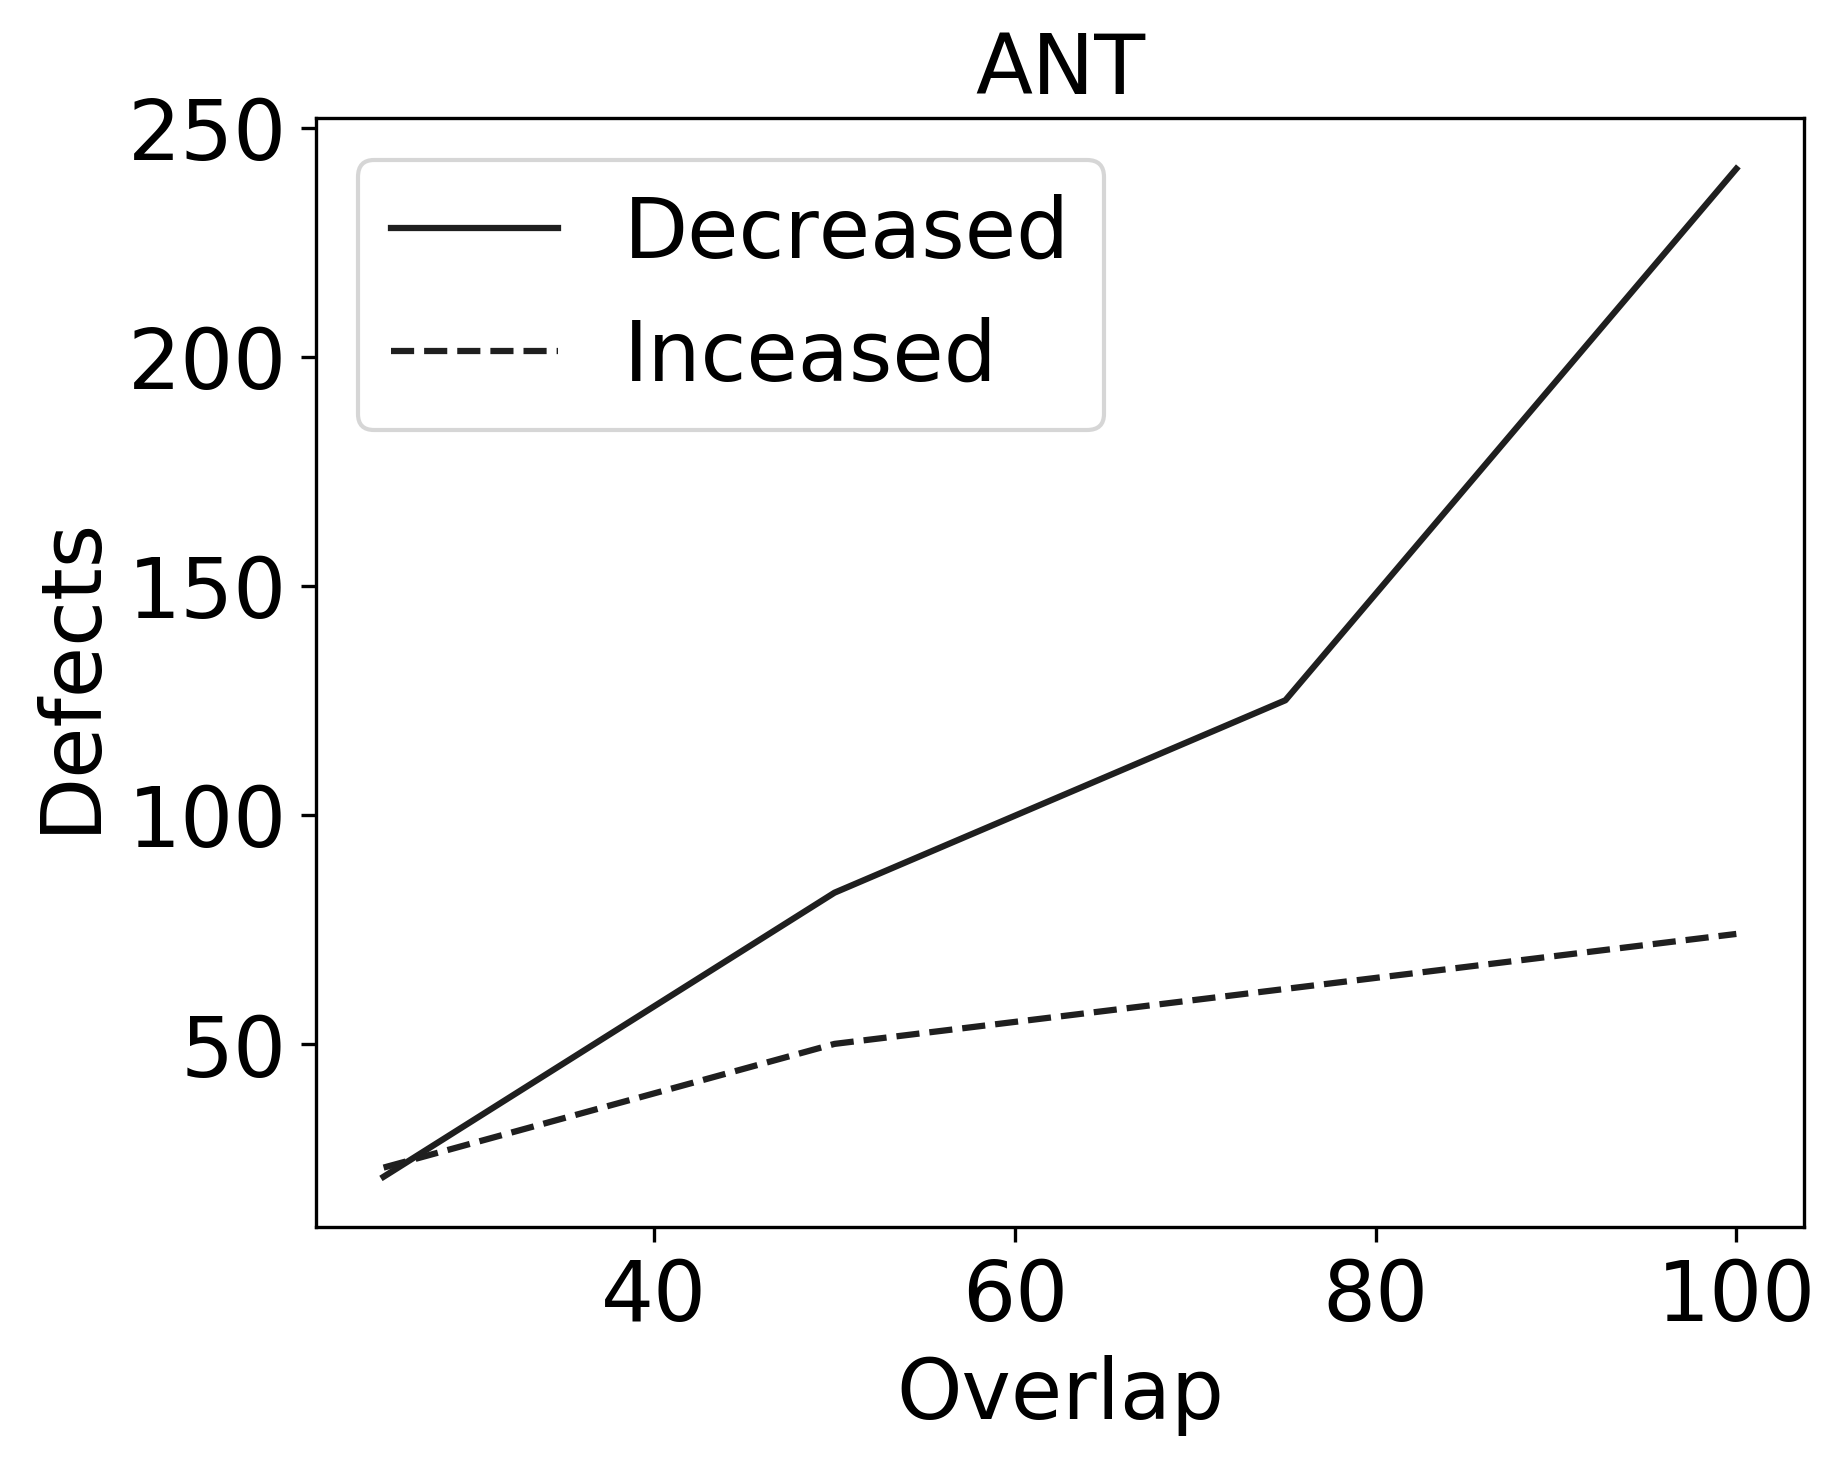
\includegraphics[width=0.7\linewidth]{sample_ant.png}
\end{center}
\[
\mathit{AUPEC} = \int_{0}^{1} f(x) \, dx \hfill
\]
\[\approx \tfrac{\Delta x}{3}\left(f(x_0) + 4f(x_1)+2f(x_2)+\cdots+4f(x_{n-1}) + f(x_{n})\right)
\]
Here, the variable $x$ represents the overlap between plans and developer changes
and  $f(x)$ represents the number of defects reduced as result of the overlap.\\

We should interpret AUPEC as follows:
\begin{enumerate}
    \item \textit{Defects Reduced:}
  AUPEC is always greater than zero and 
    \textit{larger values} of AUPEC point to \textit{more defects reduced} with increasing overlap.
    
        \item \textit{Defects Increased:}  AUPEC is still always greater than zero
        and \textit{smaller values} of AUPEC point to \textit{less defects increased} with increasing overlap.
   
\end{enumerate}
In the above plot, we show an example of XTREE on Ant. We see that the more developers used our plans (and moved right across the x-axis), then subsequent changes to the code removed far more defects than it added.  

Note: Since the actual number of defects vary from one project to another, we report the AUPEC score as a percentage of theoretical best. The theoretical best for AUPEC for defects reduced will be 100\% and 0\% for defects increased.
 
% On the other hand, in the right-hand-side figure,  when we look at defects \textit{increased}, XTREE still has a larger number of defects increased than other planners; but, the number of defects reduced in comparison to defects increased is significantly larger. Therefore, overall, we may assert that XTREE is a better planner.
\\\hline
\end{tabular}
\caption{ AUPEC = Area Under Planner Effectiveness Curve.}
\label{fig:report_sample}
\end{figure}